% !TEX root = Projektdokumentation.tex

Mobile Quiz ist eine Online Plattform, um Quizzes zu erstellen und zu lösen. Der Zugriff erfolgt via Computer oder Smartphone über einen Web-Browser. Die Plattform wird in verschiedenen HSR-Modulen (Computernetze, Informations- und Codierungstheorie, Informationssicherheit) und Weiterbildungskursen regelmässig eingesetzt. Die erste Version entstand 2012 aus einer Bachelorarbeit und wurde seither mehrmals erweitert. 

\bigskip

Vor allem Dozenten nutzen Mobile Quiz, um für Ihre Studenten Quizzes in Form von Lernhilfen während des Semesters anzubieten. Es besteht weiter die Möglichkeit die Quizzes entweder mit dem Typ Testatbedingung oder als Typ Prüfung zu erstellen und durchzuspielen. Die Wichtigsten Interaktionen mit dem Mobile Quiz - System zeigt die folgende Abbildung.

\begin{figure}[H]
	\centering
	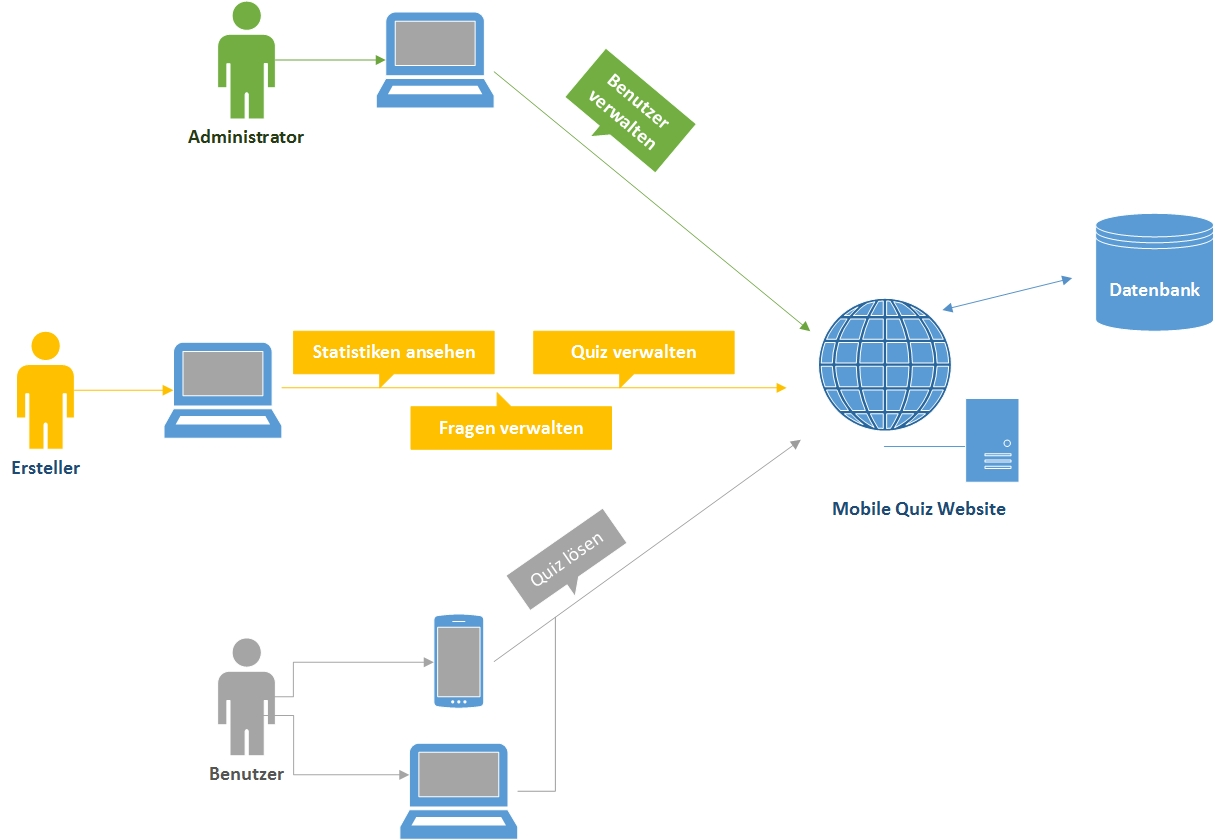
\includegraphics[width=1\textwidth]
	{Images/InteraktionMobileQuiz.jpg}
	\caption{Übersicht der wichtigsten Funktionen von Mobile Quiz}
\end{figure}

\bigskip
Die zu Beginn der Arbeit vorliegende Version umfasste zwar viele praktische Funktionen und Einstellungsmöglichkeiten, es mangelte aber an der Bedienbarkeit. Im Rahmen dieser Studienarbeit sollten deshalb einerseits die Benutzerfreundlichkeit erhöht und andererseits neue Funktionen hinzugefügt werden.

\bigskip

Das Vorgehen um sich in das Thema einzuarbeiten wurde wie folgt gewählt. In einem ersten Schritt wurde Mobile Quiz gründlich untersucht. Mit einem \gls{Usability-Test} wurden danach Optimierungsmöglichkeiten für Quizteilnehmer bestimmt. Durch die Behebung von gefunden Fehlern aus der eigenen Untersuchung machte man sich mit dem Code und den eingesetzten Technologien vertraut. Im Rahmen einer Umfeldanalyse wurden ähnliche Online-Quiz Plattformen gesucht, getestet und bewertet. Die aus den vorangegangenen Projektphasen gewonnenen Erkenntnisse halfen bei der Neugestaltung der Seiteninhalte sowie bei der Festlegung von neuen Funktionen. Beim Entwurf des Design wurden die anzuzeigenden Informationen bewusst auf das Nötigste beschränkt. Die Implementierung des Desings und der Konzepte erfolgte während fünf Wochen. Da es sich bei dieser Arbeit um eine Erweiterung eines bestehenden Systems handelt, wurden die Technologien nicht neu gewählt. Es wurde die bereits bestehende Lösung mit PHP, JavaScript und JQuery für die Logik, der MySQL Datenbank für das Speichern der Daten und HTML zusammen mit CSS für die Darstellung verwendet. Nach der Implementierungsphase wurde die Arbeit mit einem zweiten Usability-Test abgeschlossen.

\bigskip

Als Ergebnis dieser Arbeit konnte eine sowohl für den Quiz-Ersteller wie auch für den Teilnehmer wesentlich verbesserte Bedienbarkeit erreicht werden. Die Schritt-für-Schritt Benutzerführung erleichtert das Erstellen von Quizzes, Fragen und Durchführungen. Dank der überarbeiteten Excel-Vorlage können Fragen auch unterwegs, ohne eine Verbindung zum Internet, leicht erfasst und später hochgeladen werden. Durch die Erweiterung \glqq Fragen mit Bildern\grqq sind attraktivere Fragestellungen möglich. Die Konzeptänderung, welche pro Quiz mehrere Durchführungen möglich macht, erleichtert den Einsatz von Mobile Quiz im Unterricht mit mehreren Übungsgruppen. 

Mit Hilfe des neuen Designs sollten sich die Quizteilnehmer zudem schneller zurechtfinden. Dies belegt der Vergleich der Ergebnisse der beiden Usability-Tests vor und nach der Überarbeitung der Online Plattform. 

\bigskip

Die jetzt vorliegende Mobile Quiz Version wird ab dem nächsten Semester produktiv eingesetzt. Die Umsetzung der in der Analysephase ausgearbeiteten statistischen Auswertungen sowie weiteren Konzepten könnte im Rahmen einer weiteren Studienarbeit erfolgen.